\section{Identification du sens du résultat}


\subsection{Contexte}

\begin{frame}[t]{\mysubsectiontitle}
	Restriction du problème d'identification des demandes
\begin{itemize}	\small
	\item Uniquement les décisions à une demande de la catégorie
	\begin{itemize}\scriptsize
		\item Raison: plus de $50\%$ des documents dans la majorité des catégories
	\end{itemize}
	\item Classification binaire (éviter les subtilités de rédaction)
	\begin{itemize} \scriptsize
		\item Raison: les demandes sont en majorité \textbf{acceptées} ou \textbf{rejetées}
	\end{itemize}
\end{itemize}
\centering 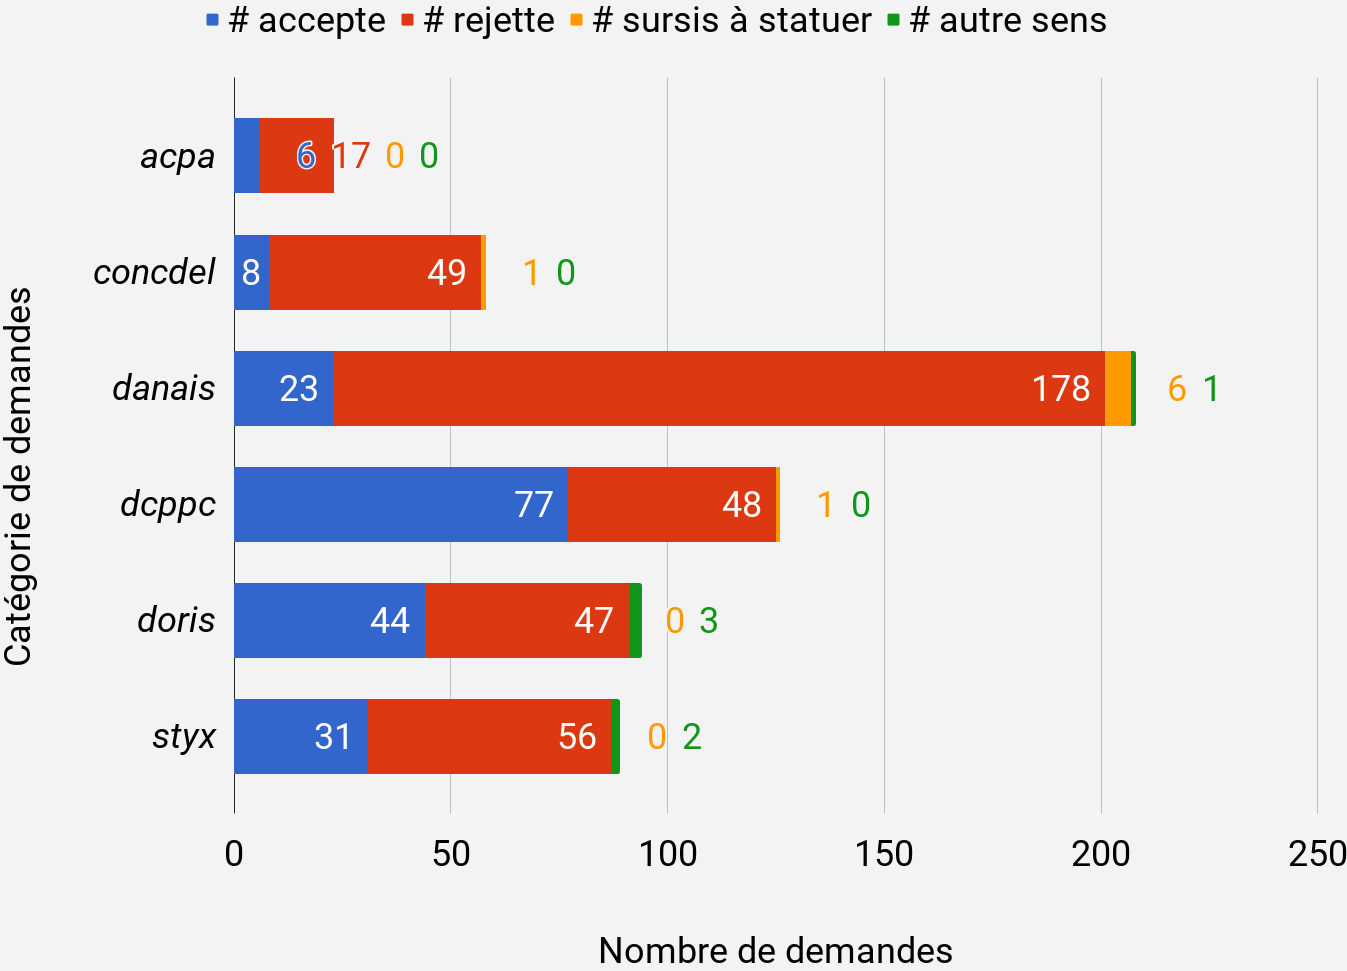
\includegraphics[width=0.7\textwidth]{chartDistrSens.png}
\end{frame}

\begin{frame}[t]{\mysubsectiontitle}
	Plusieurs algorithmes classiques existent
	\begin{itemize} \small
		\item Classifieur bayésien naïf \cite{duda1973patternclass} 
		\item K-plus-proches-voisins \cite{cover1967knn}
		\item SVM \cite{vapnik1995statlearning}
		\item Arbre de décision
		\item Analyse discriminante linéaire \cite{fisher1936linearDA} et quadratique \cite{McLachlan1992DiscrAnalyStatPattRecog-QDA}
		\item Logit-PLS \cite{tenenhaus2005logitpls}
		\item NBSVM \cite{wang2012nbsvm}
		\item fastText \cite{grave2017fasttextcls}
		\item etc.	
	\end{itemize}
\end{frame}


\subsection{Méthodes proposées : adaptations de la régression Gini-PLS}

\begin{frame}[t]{\mysubsectiontitle}
Régression Gini-PLS
\begin{itemize}\small
	\item PLS \cite{wold1966pls} (régression partielle des moindres carrés) 
	\begin{itemize}\scriptsize
		\item Réduction supervisée de dimensions $x_1, x_2, ..., x_m$ en composantes orthogonales $t_1, ...., t_h$
		
		\[t_h = \sum_{k=1}^m w_{hk}\cdot \hat{U}_{(h-1)k}\] 
		
		avec $\hat{U}_{0k} = x_{k}$, $\forall h > 0, \hat{U}_{hk}$ est le résidu de la régression de $x_k$ sur $t_1, ..., t_{h-1}$ 
		
		et $w_{hj} = \frac{\cov(\varepsilon_h, \hat{U}_{(h-1)j})}{\sqrt{\sum_{j=1}^m cov^2(\varepsilon_h, \hat{U}_{(h-1)j})}}$ (solution de $\max \cov(y,w_hX)$ s.c. $\| w_h\|=1$)
		\item Régression de la variable dépendante $y$ dans l'espace réduit
		\[y=c_1 t_1 + ... + c_h t_h + \varepsilon_h\]			
		%\item intérêt : robustesse au problème de haute dimension et élimination du pro
	\end{itemize}
	\item Gini-PLS  \cite{mussard2018ginipls}
	\begin{itemize} \scriptsize
		\item Remplacement de la covariance $\cov(x_j, y)$ par la covariance de Gini $\cog(y; x_j) := \cov(y; R(x_j))$
		\item Élimination de la sensibilité du PLS aux valeurs aberrantes
	\end{itemize}	 	
	
\end{itemize} 
\end{frame}

\begin{frame}[t]{\mysubsectiontitle}
	Algorithmes proposés {\scriptsize (en cours de rédaction pour la revue \textit{\textbf{Stats}})}
\begin{itemize} \small
\setlength\itemsep{1.5em}

\item Gini-PLS généralisé
\begin{itemize} \scriptsize
	\item Utilisation de l'opérateur co-Gini généralisé : \[\cog_\nu(x_\ell,x_k) := -\nu \cov(x_\ell,r_{k}^{\nu-1}) ; \ \nu > 1\] où $r_{k}$ est le vecteur rang décroissant de la variable $x_k$
	
	\item $\nu$ contrôle le compromis entre l'atténuation de la variabilité des variables ($\nu \rightarrow 1$) et l'influence des queues de distributions ($\nu \rightarrow \infty$)	
\end{itemize}

%\item Logit-PLS:  $\forall j > 1$, les $w_{hj} $ sont les coefficients de la régression logistique de $y$ sur les composantes $t_1, ..., t_{h-1}, u_{(h-1)j}$ \cite{tenenhaus2005logitpls}

\item Logit-Gini-PLS  généralisé : 
\begin{itemize} \scriptsize
	\item Estimation des $w_{hj}$ à partir du paramètre $\beta$ de $P(y_i = 1 / X = X_i) = \frac{\exp\left\{X_i \beta \right\}}{1+\exp\left\{ X_i \beta \right\}}$, où $X_i$ étant une observation
	\[w_j = \frac{\beta_j}{\| \beta\|}\]	
	\item les $\hat{U}_{(h)j}$ toujours estimé avec le co-Gini généralisé
\end{itemize} 
\end{itemize}
\end{frame}


\subsection{Résultats expérimentaux}

\begin{frame}[t]{\mysubsectiontitle}
	Comparaison des classifieurs PLS aux classifieurs classiques

	\scriptsize
	\centering
	\begin{tabular}{|l|l|l|l|}
		\hline
		{Représentation} & {Algorithme} & {$F_{1}$} & $F_{1_\text{arbre}} - F_1$  \\ \hline
		
		$tf-gss$ & Arbre & 0.668 & 0\\ \hline
		$tf - avg_{global}$ & LogitPLS & 0.648 & 0.02   \\ \hline
		$tf - avg_{global}$ & StandardPLS & 0.636 & 0.032  \\ \hline
		$tf - \Delta_{DF}$ & GiniPLS & 0.586 & 0.082  \\ \hline
		$tf - \Delta_{DF}$ & GiniLogitPLS & 0.578 & 0.09  \\ \hline
		- & NBSVM & 0.494 & 0.174   \\ \hline
		- & fastText & 0.412 & 0.256  \\ \hline
	\end{tabular}	

\end{frame}

\begin{frame}[t]{\mysubsectiontitle}
	Amélioration de la classification par restriction du document

	\tiny
	\centering
	
	\begin{tabular}{|c|l|l|l|c|}
		\hline
		{Catégorie} & \multicolumn{1}{c|}{Zone} & \multicolumn{1}{c|}{Représentation} & \multicolumn{1}{c|}{Algorithme} & $F_1$ \\ \hline
		\multirow{3}{*}{\textit{acpa}} & \textbf{demande\_resultat\_a\_resultat\_context} & $tf-dbidf$ & \textbf{Arbre} & \textbf{0.846} \\ 
		& litige\_motifs\_dispositif & $tf-dbidf$ & StandardPLS & 0.697 \\ 
		& litige\_motifs\_dispositif & $tf-avg_{global}$ & LogitPLS & 0.683 \\ \hline
		
		\multirow{3}{*}{\textit{concdel}} & \textbf{litige\_motifs\_dispositif} & \textbf{$tf-gss$} & \textbf{Arbre} & \textbf{0.798} \\ 
		& motifs & $tf-idf$ & GiniLogitPLS & 0.703 \\ 
		& context & $logave-dbidf$ & StandardPLS & 0.657 \\ \hline
		
		\multirow{3}{*}{\textit{danais}} & \textbf{demande\_resultat\_a\_resultat\_context} & \textbf{$avg_{local}-\chi^2$} & \textbf{Arbre} & \textbf{0.813} \\ 
		& demande\_resultat\_a\_resultat\_context & $atf-avg_{global}$ & LogitPLS & 0.721 \\ 
		& demande\_resultat\_a\_resultat\_context & $atf-avg_{global}$ & StandardPLS & 0.695 \\ \hline
		
		\multirow{3}{*}{\textit{dcppc}} & \textbf{demande\_resultat\_a\_resultat\_context} & $tf-\chi^2$ & \textbf{Arbre} & \textbf{0.985} \\ 
		& demande\_resultat\_a\_resultat\_context & $tf-\chi^2$& LogitPLS & 0.94 \\ 
		& litige\_motifs\_dispositif & $tp-mar$ & StandardPLS & 0.934 \\ \hline
		
		\multirow{3}{*}{\textit{doris}} & \textbf{litige\_motifs\_dispositif} & $tp-dsidf$ & \textbf{GiniPLS} & \textbf{0.806} \\
		& litige\_motifs\_dispositif & $tp-dsidf$ & GiniLogitPLS & 0.806 \\
		& litige\_motifs\_dispositif & $atf-ig$ & StandardPLS & 0.772 \\ \hline
		
		\multirow{3}{*}{\textit{styx}} & \textbf{motifs} & $tf-dsidf$ & \textbf{Arbre} & \textbf{1} \\ 
		& demande\_resultat\_a\_resultat\_context & $logave-dsidf$ & GiniLogitPLS & 0.917 \\ 
		& litige\_motifs\_dispositif & $tf-rf$& GiniPLS & 0.833 \\ \hline
	\end{tabular}
	
\end{frame}